\documentclass[a4paper,10pt]{IEEEtran}
\usepackage{mathptmx}

\usepackage{tabularx} % extra features for tabular environment
\usepackage{amsmath}  % improve math presentation
\usepackage{float}
% \usepackage{pdfpages}

\usepackage{subfig}

\usepackage{graphicx} % takes care of graphics including machinery
\graphicspath{ {./figures_final/} }
%\usepackage[margin=1in,letterpaper]{geometry} % decreases margins
%\usepackage{cite} % takes care of citations
\usepackage[final]{hyperref} % adds hyperlinks inside the generated pdf file
\hypersetup{
    colorlinks=true,       % false: boxed links; true: colored links
    linkcolor=blue,        % color of internal links
    citecolor=blue,        % color of links to bibliography
    filecolor=magenta,     % color of file links
    urlcolor =blue         
}
\usepackage[margin = 1in,headsep=0.5cm,headheight=2cm,letterpaper]{geometry} 

\usepackage{fancyhdr}
\pagestyle{fancy}
\lhead{Student 1 : Ahmet Akman 2442366 \\ Student 2: Kaan Demirkoparan 2442903}
\rhead{Date: \today \\ Group: Friday Morning - 6} 
%\cfoot{center of the footer!}
%\renewcommand{\headrulewidth}{0.1pt}

\title{  EE313 Fall 2022 Project Work  \protect\\ Final Report}
\author{ Ahmet Akman 2442366 -- Kaan Demirkoparan 2442903 }
\date{}
\begin{document}
\thispagestyle{empty}


\maketitle
%\tableofcontents
%\begin{abstract}
%abstract
%\end{abstract}

\section{Introduction}
Our project in the fall semester of 2022 aimed to transmit an audio signal via an optical transmitter module. It was divided into two components: the transmitter and receiver. To measure signal strength, we combined the audio signal with a reference signal. Our design featured circuit designs such as low-pass and high-pass filters, an automatic gain control circuit, and a power amplifier for the speaker. This report will give details on the project's specifications, components, and stages. It will also provide information on the design methodology, simulation results, experimental results, a comparison of the simulation and experimental results, and explanations for any differences.
\section{General Structure and Design Philisophy}
 The general structure is given in Figure \ref{general}
\begin{figure}[htbp!]
    \centering
    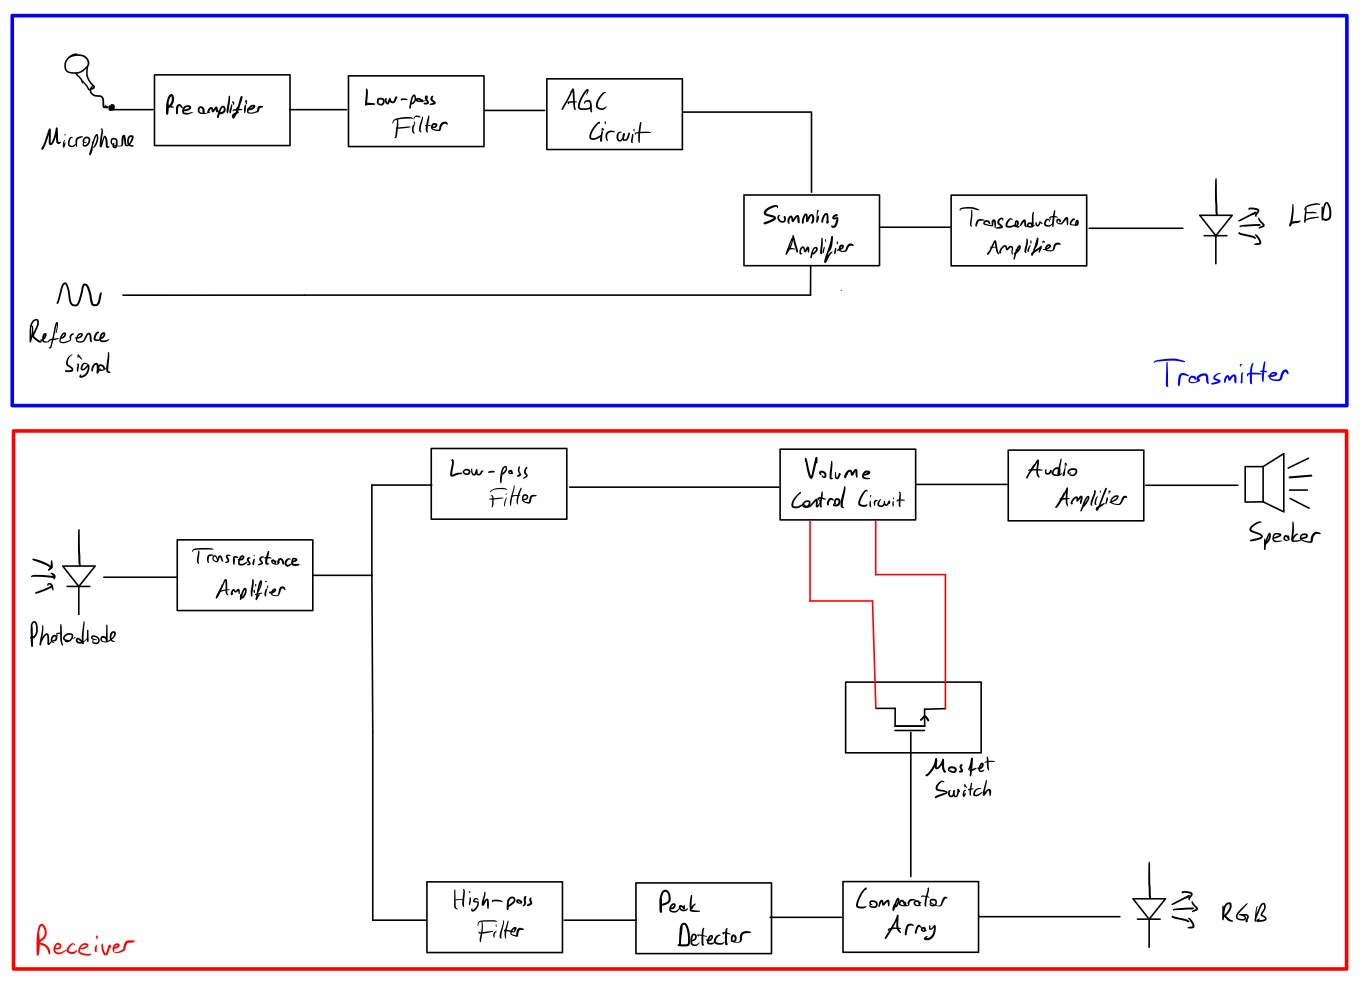
\includegraphics[width = 1\linewidth]{general_structure.jpeg}
    \caption{General Structure}
    \label{general}
\end{figure} 
\section{Transmitter Side}
\subsection{Input and Early Stage Amplification}
The microphone functions as a resistor, with its resistance varying based on the audio waves. To turn audio signals into electrical signals, a voltage divider circuit can be employed. However, the resulting output signal is quite weak, making it susceptible to noise. To mitigate this, the small signal is amplified using a common source or common emitter amplifier, which results in a less noise-sensitive and more usable voltage range signal. Subsequently, this signal is passed through a low pass filter to separate the human voice for further processing. The schematic of this circuit is given in Figure \ref{PreAmp}

\begin{figure}[htbp!]
    \centering
    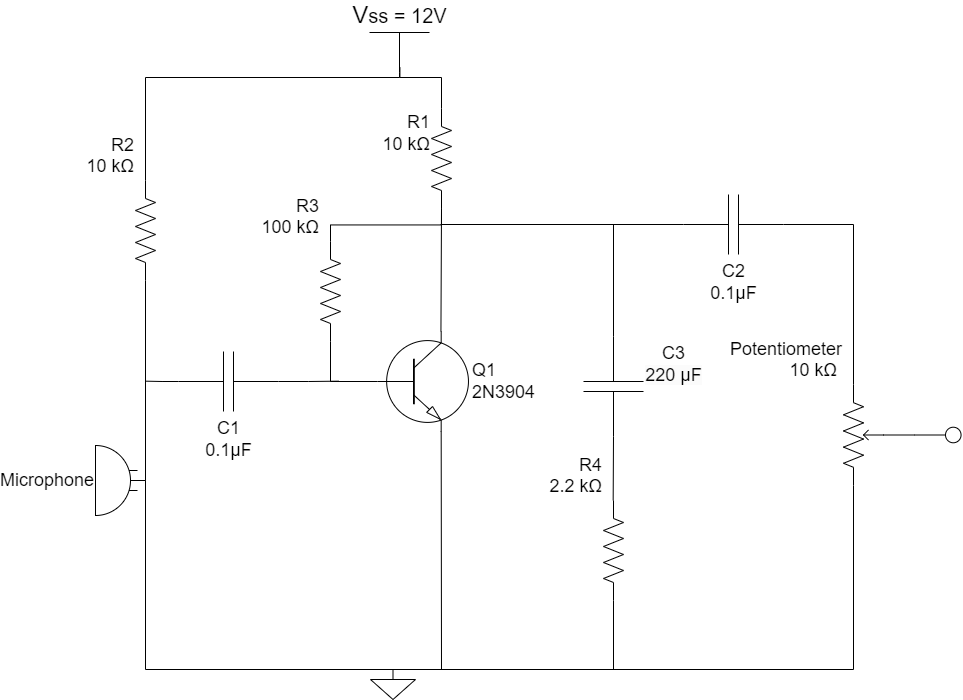
\includegraphics[width = 1\linewidth]{Preamplifier.drawio.png}
    \caption{Microphone and preamplification circuit}
    \label{PreAmp}
\end{figure} 
The amplification factor can be adjusted from the pot so that the voice level and noise level can be fine tuned with a proper selection of amplification factor. The construction of this circuit is done on a breadboard and it can be said that the design specs are satisfied successfully as shown in the demonstration. 
\subsection{Low Pass Filter}
After the preamplification process is completed, the resulting output signal is sent to a low-pass filter to remove any unwanted frequencies. The typical range of human hearing is between 20 Hz and 20 kHz, but for this specific project, only the range of 100 Hz to 5 kHz is used. This is done to prevent overlap between the audio signal and the reference signal in the frequency domain. The low-pass filter used in this project is a two stage sallen-key active low pass filter which is shown in Figure \ref{lowpass}
\begin{figure}[htbp!]
    \centering
    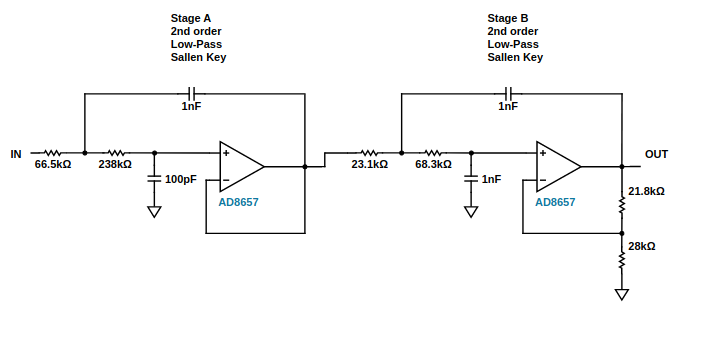
\includegraphics[width = 1\linewidth]{active_low_pass_circuit.png}
    \caption{Active low pass filter.}
    \label{lowpass}
\end{figure} 
The frequency response of the circuit is given in Figure \ref{lowpass_resp}.
\begin{figure}[htbp!]
    \centering
    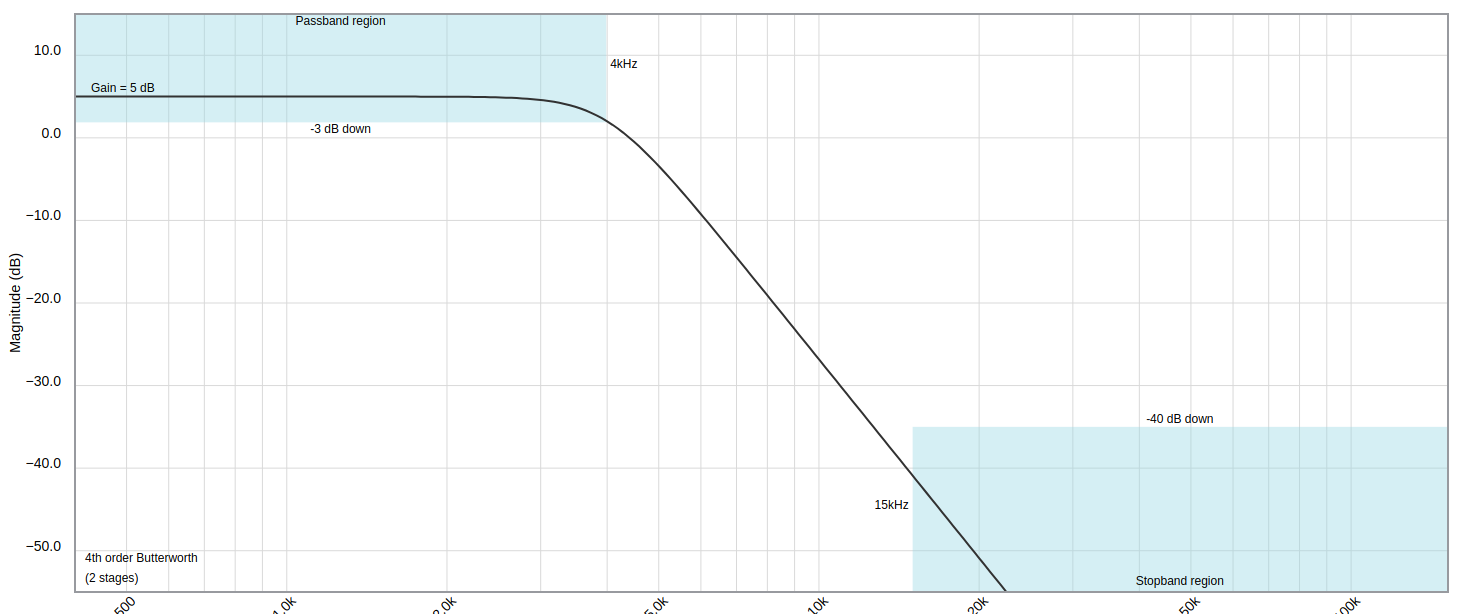
\includegraphics[width = 1\linewidth]{active_low_pass.png}
    \caption{Active low pass filter frequency response.}
    \label{lowpass_resp}
\end{figure} 
The filtering strategy is observed to be pretty accurate decision as very small noise is heard from the output. 
\subsection{Automatic Gain Control}
The automatic gain control circuit given in Figure \ref{AGC} is designed.

\begin{figure}[htbp!]
    \centering
    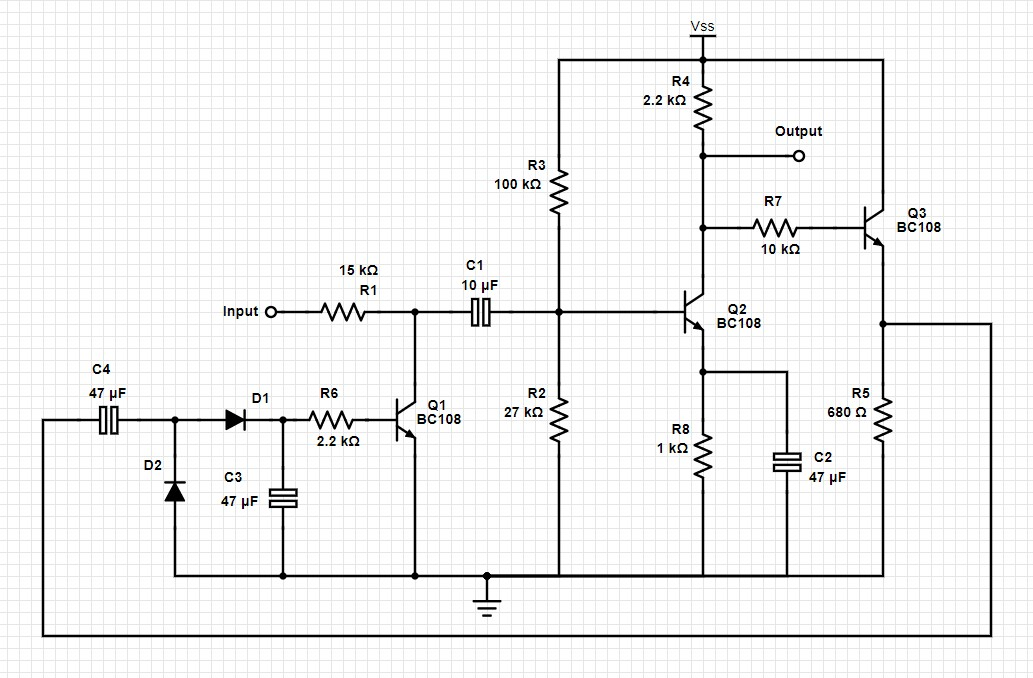
\includegraphics[width = 1\linewidth]{AGC Circuit.jpg}
    \caption{Automatic gain circuit schematic.}
    \label{AGC}
\end{figure} 
 The circuit composed of three transistors. The first stage (Q2) is a common emitter amplifier with a feedback supplied by other two transistor. The second transistor in common collector configuration is a voltage buffer that takes the amplitude information of the Q2. Then the Q3 works as an active resistor which takes input from a simple peak detector connected after Q3. The simulation results are given in Figure \ref{AGC_sim} .
 \begin{figure}[htbp!]
    \centering
    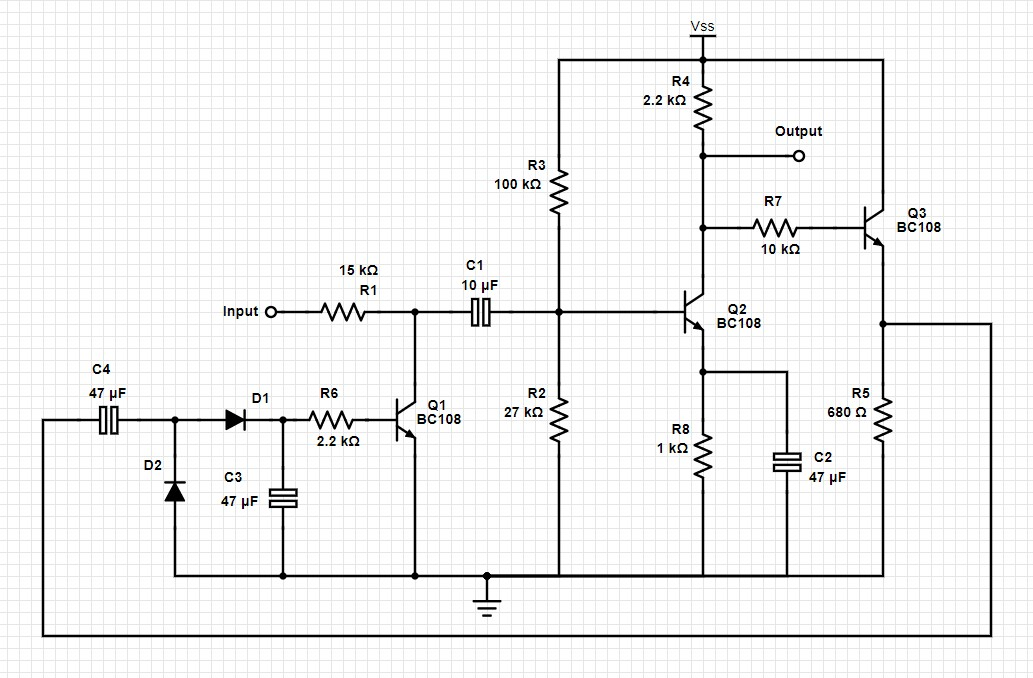
\includegraphics[width = 1\linewidth]{AGC Circuit.jpg}
    \caption{Automatic gain circuit simulation.}
    \label{AGC_sim}
\end{figure} 

\subsection{Reference Signal Summation}

The constant gain audio signal and the high-frequency reference signal should be summed before transmission. This summation process is thought to be applied by adopting a simple op-amp summing amplifier.  The schematic is given in \ref{summing} is used in 1 to 1 ratio.
\begin{figure}[htbp!]
    \centering
    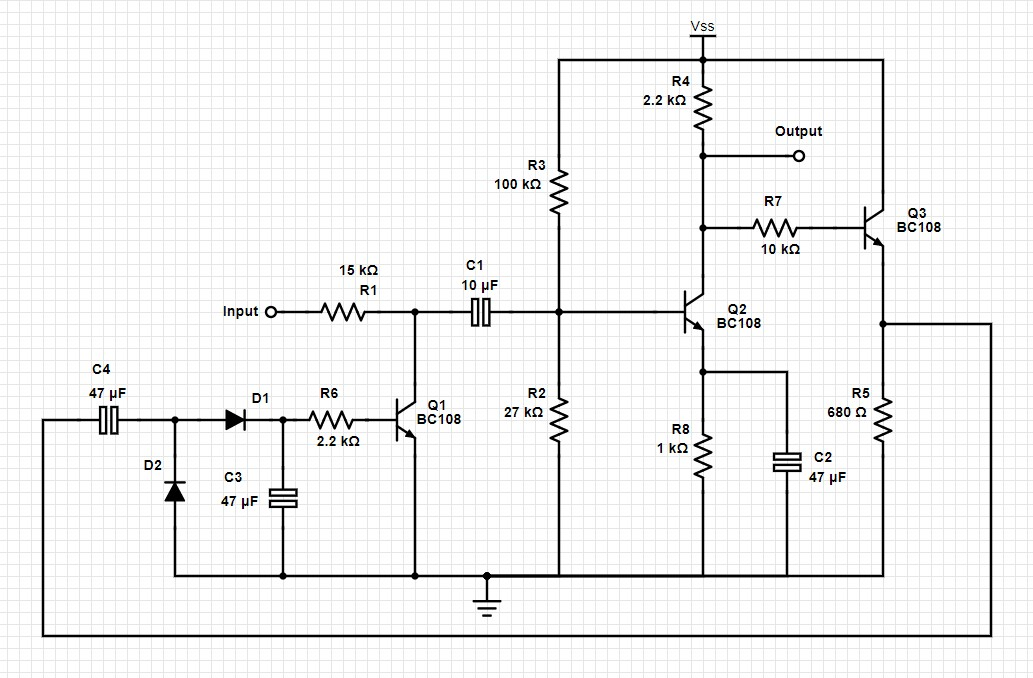
\includegraphics[width = 1\linewidth]{AGC Circuit.jpg}
    \caption{Summing amplifier.}
    \label{summing}
\end{figure} 
This circuit is a basic sum operator and 
\subsection{Light Transmission}
The decision on the light transmission is made towards using an IR LED. Since the LED's brightness changes with respect to the current pass thorugh it , we needed to convert the signal from voltage form to current form. In order achieve this we have utilized a transconductance amplifier given in Figure \ref{transconductance}. 
\begin{figure}[htbp!]
    \centering
    \includegraphics[width = 1\linewidth]{Led Driver Circuit.jpg}
    \caption{Transconductance amplifier.}
    \label{transconductance}
\end{figure} 
The circuit is composed of a basic degenerated common emitter configuration with a feedback. 

As a result of our prototyping process, we have constructed the circuit on a breadboard and the transmitter part of the circuit is successfully operated as expected without any big surprise. The physical structure of our prototype is given in Figure \ref{transmitter_breadboard}
\begin{figure}[htbp!]
    \centering
    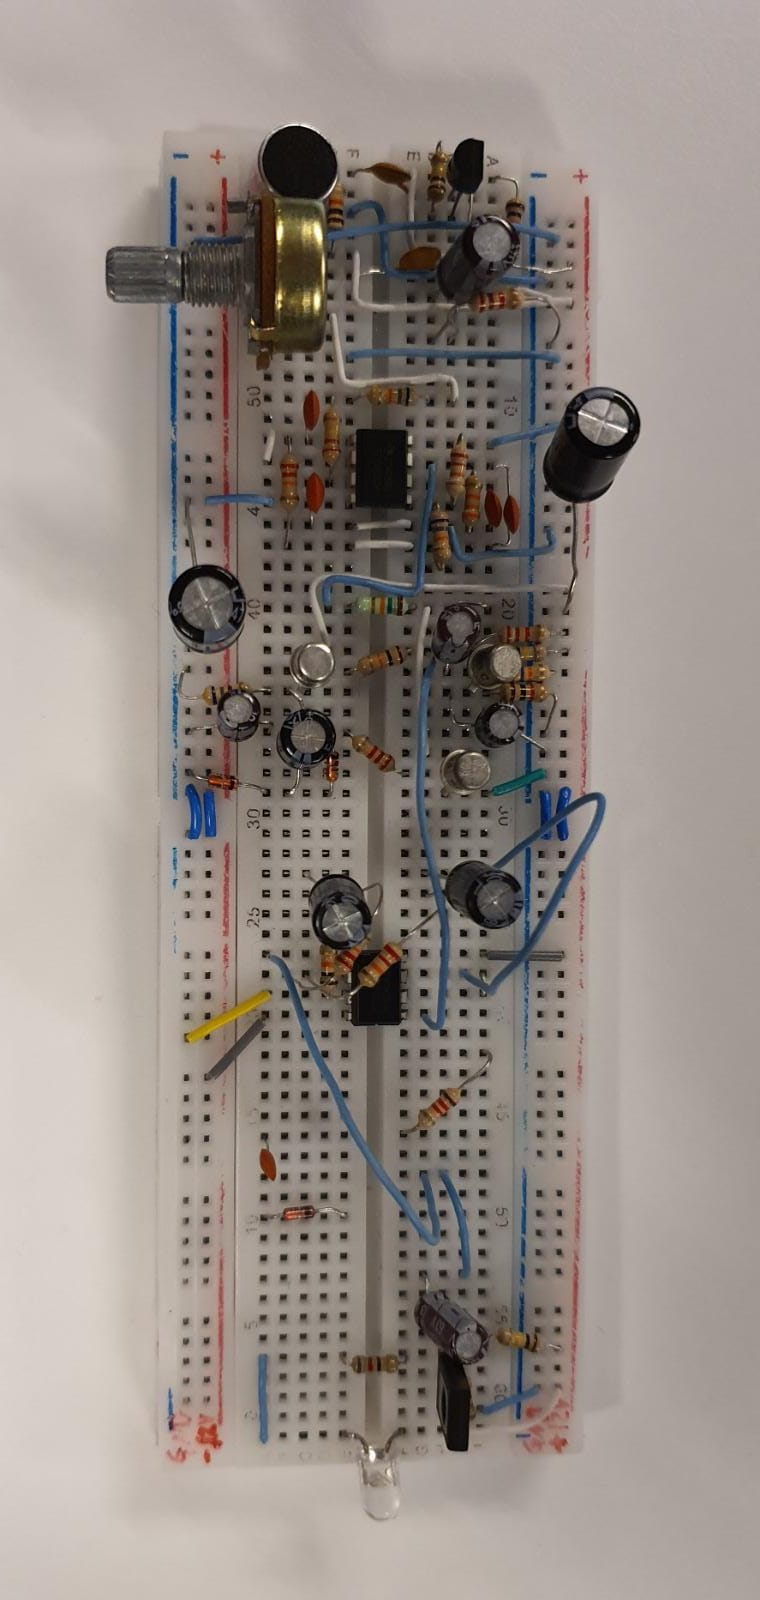
\includegraphics[width = 1\linewidth]{transmitter.jpeg}
    \caption{Transmitter prototype.}
    \label{transmitter_breadboard}
\end{figure} 

\section{Receiver Side}
\subsection{Light Receiver}
\subsection{Voice Signal Path}
\subsubsection{Low Pass Filter}
\subsubsection{Speaker Driver}
\subsection{Carrier Signal Path}
\subsubsection{High Pass Filter}
\subsubsection{Signal Level Indication}


\section{Conclusion}

\section*{Appendix}

\end{document}

%%%%%%%%%%%%%%%%%%%%%%   EXAMPLE TABLE   %%%%%%%%%%%%%%%%%%%%%%%%%%%%%%%%
\begin{table}[H]
\begin{center}
    \caption{Resistance reading by color code convention.}
    \vspace{2mm}
    \begin{tabular}{||c | c | c||} 
        \hline
        Color Order & Value & Tolerance \\ [0.5ex] 
        \hline\hline
        Brown / Black / Red / Gold & 1k\( \Omega \) & \( \% \) 5  \\ 
        \hline
        Yellow / Violet / Red / Gold & 4.7k\( \Omega \) & \( \% \) 5   \\
        \hline
        Brown / Grey / Orange / Gold & 18k\( \Omega \) & \( \% \) 5  \\ [1ex] 
        \hline
    \end{tabular}
\end{center}
\end{table}


%%%%%%%%%%%%%%%%%%%%%%   EXAMPLE IMAGE   %%%%%%%%%%%%%%%%%%%%%%%%%%%%%%%%
\begin{figure}[H]
\centering
\includegraphics[width = 0.75\linewidth]{5.png}
\caption{Circuit schematic for the step 5}
\end{figure} 

%%%%%%%%%%%%%%%%%%%%%%   EXAMPLE IMAGE FROM PDF   %%%%%%%%%%%%%%%%%%%%%%%%%%%%%%%%
\begin{figure}[H] \centering{
    \includegraphics[scale=0.25]{2a_plot.pdf}}
    \caption{Experiment 2}
\end{figure}
%%%%%%%%%%%%%%%% Deneme Push